\setcounter{section}{15}

\section{Теорема Кантора-Бернштейна}

\par \textbf{Теорема Кантора Бернштейна: } если $A$ не более мощно чем $B$, и $B$ не более мощно чем $A$, то $A \cong B$
\par $\blacktriangle$ Если $A$ не более мощно чем $B$, то $A \cong B_1$ для некоторого $B_1 \subset B$. Обозначим через $f$ соответствующую биекцию из $A$ в $B_1$. Аналогично $B \cong A_1$ для некоторого $A_1 \subset A$, обозначим через $g$ биекцию из $B$ в $A_1$. Определим $A_2$ как $g(B_1)$. Поскольку $B_1 \subset B$, то $A_2 = g(B_1) \subset g(B) = A_1$, при этом $A_2 \cong B_1 \cong A$. Получим утверждение, эквивалентное исходной теореме: если $A_2 \subset A_1 \subset A_0$ и $A_2 \cong A_0$, то $A_1 \cong A_0$. Это утверждение мы и будем доказывать.
\par Обозначим через $h$ композицию $g \circ f$. Это биекция из $A_0$ в $A_2$. Для всех натуральных $k > 2$ определим рекурсивно $A_k$ как $h(A_{k-2})$. Также определим "слои"  $C_k$ как $A_k \setminus
A_{k+1}$. Поскольку $h$ — биекция, то $h(C_k) = C_{k+2}$ и $h$ задаёт биекцию между $C_k$ и $C_{k+2}$.
Однако не обязательно любой элемент $A_0$ войдёт в какой-то слой. Будет ещё "ядро" $C = \bigcap_{k=0}^{\infty} A_k$. Тогда $A_0 = C \cup C_0 \cup C_1 \cup C_2 \cup C_3 \cup . . .$ и $A_1 = C \cup C_1 \cup C_2 \cup C_3 \cup . . . $. Наконец,
построим биекцию $\alpha$ между $A_0$ и $A_1$:
$$\alpha(x)=\left\{
\begin{array}{ccc}
x, x \in C \cup C_1 \cup C_3 \cup C_5 \cup ...\\
h(x), \; x \in C_0 \cup C_2 \cup C_4 \cup ...\\
\end{array}
\right. $$
\par Это действительно биекция: все элементы слоёв с нечётными номерами, а также элементы ядра, остаются на месте, а все слои с чётными номерами биективно отображаются
в слои с номерами, на 2 бОльшими. Поэтому все слои, кроме нулевого, оказываются
покрыты. Таким образом, эквивалентное утверждение, а с ним и исходная теорема,
доказаны. $\blacksquare$

\begin{figure}[h]
\center{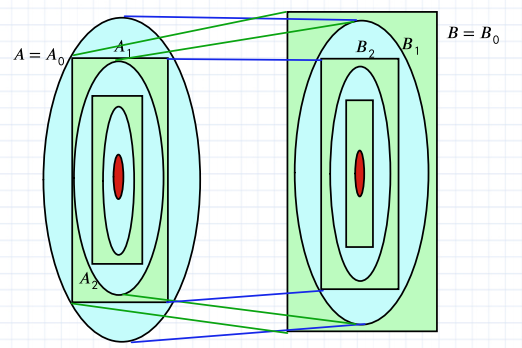
\includegraphics[width=0.5\textwidth]{images/16.png}}
\end{figure}